\documentclass[10pt]{article}
\textwidth 6.5in
\textheight 9in
\oddsidemargin -0.2in
\topmargin -0.5in
 
\usepackage{graphicx,times,amsmath} % Add all your packages here
\usepackage[all]{xy}
\usepackage{multirow}
\usepackage{graphicx}
\usepackage{color}
\usepackage{tabularx}
\usepackage{url}
\usepackage{amsmath}
\usepackage{amssymb}
\usepackage{multirow}
\usepackage[noend,ruled,linesnumbered]{algorithm2e}
\usepackage[numbers, sort]{natbib}
\usepackage{listings}
\usepackage[svgnames]{xcolor}
%\usepackage{newtxtext}
\definecolor{javared}{rgb}{1,0,0} % for strings
\definecolor{javagreen}{rgb}{0.25,0.5,0.35} % comments
\definecolor{javapurple}{rgb}{0.5,0,0.35} % keywords
\definecolor{javadocblue}{rgb}{0.25,0.35,1} % javadoc
\lstdefinestyle{highlight} {
moredelim=[is][\bfseries\textcolor{javadocblue}]{<<>>}{>><<},
moredelim=[is][\itshape]{!!}{??}
}
\lstset{language=Python,
  keywordstyle=\color{javapurple}\bfseries,
  stringstyle=\color{javared},
  commentstyle=\color{javagreen},
  basicstyle=\tt\small,        % the size of the fonts that are used
                               % for the code
  style=highlight,
  breakatwhitespace=false,         % sets if automatic breaks should only happen at whitespace
  breaklines=true,                 % sets automatic line breaking                   % sets the caption-position to bottom
  extendedchars=true,              % lets you use non-ASCII characters; for 8-bits encodings only, does not work with UTF-8
  showspaces=false,                % show spaces everywhere adding particular underscores; it overrides 'showstringspaces'
  showstringspaces=false,          % underline spaces within strings only
  showtabs=false,                  % show tabs within strings adding particular underscores
  tabsize=2,                     % sets default tabsize to 2 spaces
  numbers=left,
  %frameround=ftff,
  frame=shadowbox,
  rulecolor=\color{black},
  rulesepcolor=\color{gray}
  }
\usepackage{hyperref}
\hypersetup{
    colorlinks=true,
    citecolor=teal,
    linkcolor=olive, % Internal links, those generated by cross-referenced elements    
    urlcolor=blue % Links to web sites
}
\newcommand{\sbol}[1]{\textbf{#1}}

\begin{document}
  \setlength{\parindent}{1em}
  \setlength{\parskip}{0em}
  \setlength{\parsep}{0em}

\section*{A brief description of the CRISPR circuit using SBOL 2.0 data model}
We first give a brief description of the CRISPR-based repression module. We use bold font in the following text and figure captions to mark available data model in SBOL 2.0. Detailed description of properties of the data model is available in the~\href{http://sbolstandard.org/downloads/specification-data-model-2-0/}{Specification
  (Data Model 2.0)}.

First, consider the CRISPR-based Repression Template \sbol{ModuleDefinition} shown in the center of Figure~\ref{fig:fig-CRPb}. It provides a generic description of CRISPR-based repression behavior. Namely, it includes generic \emph{Cas9}, \emph{guide RNA} (gRNA), and \emph{target} DNA \sbol{FunctionalComponent} instances. It also includes a \emph{genetic production} \sbol{Interaction} that expresses a generic target gene product.  Finally, it includes a \emph{non-covalent binding} \sbol{Interaction} that forms the Cas9/gRNA complex (shown as dashed arrows), which in turn participates in an \emph{inhibition} \sbol{Interaction} to repress the target gene product production (shown with a tee-headed arrow). The CRISPR-based Repression Template is then instantiated to test a particular CRISPR-based repression device, CRPb, by the outer CRPb Characterization Circuit \sbol{ModuleDefinition}.  This outer characterization circuit includes gene \sbol{FunctionalComponents} to produce specific products (i.e., mKate, Gal4VP16, cas9m\_BFP, gRNA\_b, and EYFP), as well as \sbol{FunctionalComponents} for the products themselves.  Next, it includes \emph{genetic production} \sbol{Interactions} connecting the genes to their products, and it has a \emph{stimulation} \sbol{Interaction} that indicates that Gal4VP16 stimulates production of EYFP.  Finally, it uses \sbol{MapsTo} objects (shown as dashed lines) to connect the generic \sbol{FunctionalComponents} in the template to the specific objects in the outer \sbol{ModuleDefinition}.  For example, the outer module indicates that the target protein is EYFP, while the cas9\_gRNA complex is cas9m\_BFP\_gRNA\_b.

\begin{center}
\begin{figure}[tbph]
  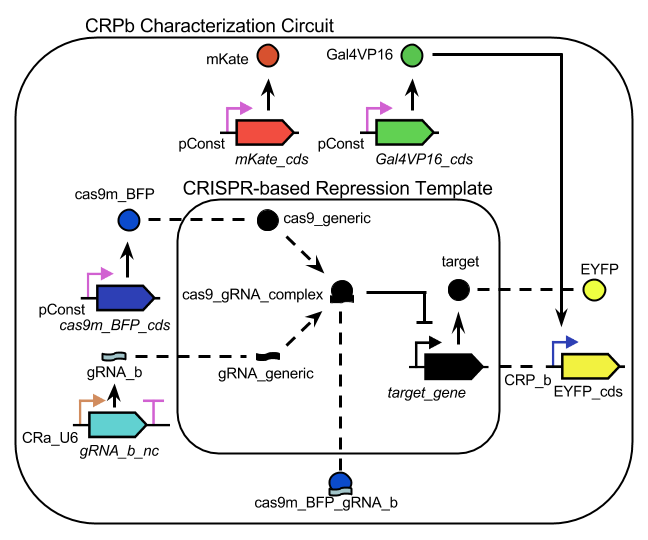
\includegraphics[width=0.95\textwidth]{figures/crispr_repression2} 
\caption{\label{fig:fig-CRPb} Illustration of a hierarchical CRISPR-based repression module represented in SBOL 2.0 (adapted from Figure~1a in \cite{kiani2014crispr}). The CRISPR-based Repression Template \sbol{ModuleDefinition} describes a generic CRISPR repression circuit that combines a Cas9 protein with a gRNA to form a complex (represented by the dashed arrows) that represses a target gene (represented by the arrow with the tee arrowhead).  These relationships between these \sbol{FunctionalComponents} (instances of \sbol{ComponentDefinitions}) are represented in SBOL 2.0 using \sbol{Interactions}.  This \sbol{Module} is instantiated in the outer CRPb Characterization Circuit \sbol{ModuleDefinition} in order to specify the precise (including \sbol{Sequences} when provided) \sbol{FunctionalComponents}  used for each generic \sbol{FunctionalComponent}. The undirected dashed lines going into the template \sbol{Module} represent \sbol{MapsTo} objects that specify how specific \sbol{FunctionalComponents} replace the generic ones.}
\end{figure}

\section*{Modeling CRISPR repression using {\tt pySBOL}}
\end{center}

\subsection*{Creating SBOL Document}
 All SBOL data objects are organized within an \sbol{SBOLDocument} object. The \sbol{SBOLDocument} provides a rich set of methods to create, access, update, and delete each type of \sbol{TopLevel} object (i.e., \sbol{Collection}, \sbol{ModuleDefinition}, \sbol{ComponentDefinition}, \sbol{Sequence}, \sbol{Model}, or \sbol{GenericTopLevel}). Every SBOL object has a \emph{uniform resource identifier} (URI) and consists of properties that may refer to other objects, including non-\sbol{TopLevel} objects such as SequenceConstraint and Interaction objects. \texttt{pySBOL} organizes the URI collections to enable efficient access
 
\vspace{\abovedisplayskip}
\begin{minipage}{0.95\textwidth} 
\begin{lstlisting}
from sbol import *

setHomespace("http://sbols.org/CRISPR_Example")
toggleSBOLCompliantTypes()
version = "1.0.0"
doc = Document()
\end{lstlisting}
\end{minipage}

The method \lstinline+setHomespace+ sets the default URI prefix to the string `http://sbols.org/CRISPR\_Example'. All data objects created following this statement carry this default URI prefix. The author of any SBOL object should use a URI prefix that either they own or an organization of which they are a member owns. Setting a default namespace is like a signature verifying ownership of objects. 

\subsection*{Adding CRISPR-based Repression Template module}
\subsubsection*{Creating \sbol{TopLevel} objects}
We first create the CRISPR-based Repression Template module shown in
Figure~\ref{fig:fig-CRPb}. In this template, we include definitions
for generic \emph{Cas9}, \emph{guide RNA} (gRNA), and \emph{target}
DNA \sbol{FunctionalComponent} instances. They are encoded as
\sbol{ComponentDefinition} objects. With \sbol{FunctionalComponent}, optional fields such as \emph{direction} are used to specify the input, output, both, or neither with regards to the \sbol{ModuleDefinition} that contains it. Creation of the generic Cas9 (line 2) \sbol{ComponentDefinition} is done by passing its \emph{displayId}
``cas9\_generic'', \emph{version} specified by the \lstinline+version+
string, and \emph{type} to the \lstinline+ComponentDefinition+
constructor. Every \sbol{ComponentDefinition} must contain one or more
types, each of which is specified by a URI. A type specifies the
component's category of biochemical or physical entity (for example
DNA, protein, or small molecule). The generic Cas9's type is
\lstinline+PROTEIN+, which is defined as the BioPAX ontology term for
protein (\url{http://www.biopax.org/release/biopax-level3.owl\#Protein}).  Finally, an optional \emph{version} specified by the \lstinline+version+ string may be specied. If \emph{version} is not specified, it will be set by default to 1.0.0
.Other \sbol{ComponentDefinition} objects shown below are created in the same
way. A \sbol{ComponentDefinition} object can optionally have one or
more roles, also in the form of URIs. The \lstinline+gRNA_generic+ has
a role of \lstinline+SGRNA+ (line 7 below), defined as the
\emph{Sequence Ontology} (SO) term ``SO:0001998''
(\url{http://identifiers.org/so/SO:0001998}) in the
library. Similarly, the \lstinline+target_gene+ on line 16 below has a role of
\lstinline+PROMOTER+, defined as SO term ``SO:0000167''
(\url{http://identifiers.org/so/SO:0000167}). We then create the \sbol{ModuleDefinition} template with the displayId ``CRISPR\_Template'' and \lstinline+version+. 

\vspace{\abovedisplayskip}
\begin{minipage}{0.95\textwidth} 
\begin{lstlisting}
#Create ComponentDefinition for cas9_generic protein
cas9_generic = ComponentDefinition("cas9_generic", BIOPAX_PROTEIN, version)
doc.addComponentDefinition(cas9_generic)

#Create ComponentDefinition for gRNA_generic RNA
gRNA_generic = ComponentDefinition("gRNA_generic", BIOPAX_RNA, version)
gRNA_generic.roles.set(SO_SGRNA)
doc.addComponentDefinition(gRNA_generic)

#Create ComponentDefinition for cas9_gRNA_complex
cas9_gRNA_complex = ComponentDefinition("cas9_gRNA_complex", BIOPAX_COMPLEX, version)
doc.addComponentDefinition(cas9_gRNA_complex)

#Create ComponentDefinition for target gene
target_gene = ComponentDefinition("target_gene", BIOPAX_DNA, version)
target_gene.roles.set(SO_PROMOTER)
doc.addComponentDefinition(target_gene)

#Create ComponentDefinition for target protein
target = ComponentDefinition("target", BIOPAX_PROTEIN, version)
doc.addComponentDefinition(target)

#Create ModuleDefinition for CRISPR_Repression_Template
CRISPR_Template = ModuleDefinition("CRISPR_Template", version)
doc.addModuleDefinition(CRISPR_Template)
\end{lstlisting}
\end{minipage}

By default, pySBOL operates in SBOL-compliant mode. In SBOL-compliant mode, each constructor creates an SBOL-compliant URI with the following form:
\begin{center}
http://$\langle$prefix$\rangle$/$\langle$displayId$\rangle$/$\langle$version$\rangle$
\end{center}
using the default URI prefix and provided displayId and version. The \emph{$\langle$prefix$\rangle$} represents a URI for a namespace (for example, {\tt www.sbols.org/CRISPR\_Example}). The author of a \sbol{TopLevel} object, such as the \sbol{ModuleDefinition} object we just created, should use a URI prefix that either they own or an organization of which they are a member owns. When using compliant URIs, the owner of a prefix must ensure that the URI of any unique \sbol{TopLevel} object that contains the prefix also contains a unique  \emph{$\langle$displayId$\rangle$} or \emph{$\langle$version$\rangle$} portion. Multiple versions of an SBOL object can exist and would have compliant URIs that contain identical prefixes and displayIds, but each of these URIs would need to end with a unique version. Lastly, the compliant URI of a non-\sbol{TopLevel} object is identical to that of its parent object, except that its displayId is inserted between its parent's displayId and version. This form of compliant URIs is chosen to be easy to read, facilitate debugging, and support a more efficient means of looking up objects and checking URI uniqueness. 

\subsubsection*{Specifying Interactions}
We are now ready to specify the interactions in the repression template. The first one is the complex formation interaction for \lstinline+cas9_generic+ and \lstinline+gRNA_generic+. We first create an \sbol{Interaction} object \lstinline+Cas9Complex_Formation+ in \lstinline+CRISPR_Template+, with the displayId ``cas9\_complex\_formation'' and a non-covalent binding type (line 1 to 4). It is recommended that terms from the \emph{Systems Biology Ontology} (SBO)~\cite{Courtot2011} are used specify the types for interactions. Table 11 of the ~\href{http://sbolstandard.org/downloads/specification-data-model-2-0/}{Specification  (Data Model 2.0)} document provides a list of possible SBO terms for the types property and their corresponding URIs. 

Next, we create three participants to this interaction object. Each participant is modeled as a \sbol{Participation} object and it refers to the corresponding \sbol{FunctionalComponent} object. For example, the \lstinline+cas9_generic_participation+ \sbol{Participation} object refers to the \lstinline+cas9_generic_fc+ \sbol{FunctionalComponent} object. Note that even if we do not specify such object, since there exists a \lstinline+cas9_generic+ \sbol{ComponentDefinition} object, and the ``createDefaults'' of this \sbol{SBOLDocuemnt} is set to \lstinline+true+, a \sbol{FunctionalComponent} with the same displayId ``cas9\_generic'' will be automatically created and it connects the reference from the \lstinline+cas9_generic_participation+ \sbol{Participation} to the \lstinline+cas9_generic+ \sbol{ComponentDefinition}. We also assign a \lstinline+REACTANT+ role to it.

\vspace{\abovedisplayskip}
\begin{minipage}{0.95\textwidth}%{\linewidth} 
\begin{lstlisting}
Cas9Complex_Formation = CRISPR_Template.interactions.create("cas9_complex_formation")
Cas9Complex_Formation.types.set(SBO_NONCOVALENT_BINDING)

cas9_generic_fc = CRISPR_Template.functionalComponents.create("cas9_generic")
cas9_generic_fc.definition.set(cas9_generic.persistentIdentity.get())
cas9_generic_fc.access.set(SBOL_ACCESS_PUBLIC)
cas9_generic_fc.direction.set(SBOL_DIRECTION_IN_OUT)
cas9_generic_fc.version.set(version)

cas9_generic_participation = Cas9Complex_Formation.participations.create("cas9_generic")
cas9_generic_participation.roles.set(SBO_REACTANT)
cas9_generic_participation.participant.set(cas9_generic_fc.identity.get())

gRNA_generic_fc = CRISPR_Template.functionalComponents.create("gRNA_generic")
gRNA_generic_fc.definition.set(gRNA_generic.persistentIdentity.get())
gRNA_generic_fc.access.set(SBOL_ACCESS_PUBLIC)
gRNA_generic_fc.direction.set(SBOL_DIRECTION_IN_OUT)
gRNA_generic_fc.version.set(version)

gRNA_generic_participation = Cas9Complex_Formation.participations.create("gRNA_generic")
gRNA_generic_participation.roles.set(SBO_REACTANT)
gRNA_generic_participation.participant.set(gRNA_generic_fc.identity.get())

cas9_gRNA_complex_fc = CRISPR_Template.functionalComponents.create("cas9_gRNA_complex")
cas9_gRNA_complex_fc.definition.set(cas9_gRNA_complex.persistentIdentity.get())
cas9_gRNA_complex_fc.access.set(SBOL_ACCESS_PUBLIC)
cas9_gRNA_complex_fc.direction.set(SBOL_DIRECTION_IN_OUT)
cas9_gRNA_complex_fc.version.set(version)

cas9_gRNA_complex_participation = Cas9Complex_Formation.participations.create("cas9_gRNA_complex")
cas9_gRNA_complex_participation.roles.set(SBO_PRODUCT)
cas9_gRNA_complex_participation.participant.set(cas9_gRNA_complex_fc.identity.get())
\end{lstlisting}
\end{minipage}

The remaining two interactions, namely the genetic production of the target protein from the \lstinline+target_gene+ and the inhibition of the target protein by the \lstinline+cas9_gRNA_complex+, are specified using the same method calls.

\vspace{\abovedisplayskip}
\begin{minipage}{0.95\textwidth}%{\linewidth} 
\begin{lstlisting}
#Production of target from target gene
EYFP_production = CRISPR_Template.interactions.create("target_production")
EYFP_production.types.set(SBO_GENETIC_PRODUCTION)

target_gene_fc = CRISPR_Template.functionalComponents.create("target_gene")
target_gene_fc.definition.set(target_gene.persistentIdentity.get())
target_gene_fc.access.set(SBOL_ACCESS_PUBLIC)
target_gene_fc.direction.set(SBOL_DIRECTION_IN_OUT)
target_gene_fc.version.set(version)

target_gene_participation = EYFP_production.participations.create("target_gene")
target_gene_participation.roles.set(SBO_PROMOTER)
target_gene_participation.participant.set(target_gene_fc.identity.get())

target_fc = CRISPR_Template.functionalComponents.create("target")
target_fc.definition.set(target.persistentIdentity.get())
target_fc.access.set(SBOL_ACCESS_PUBLIC)
target_fc.direction.set(SBOL_DIRECTION_IN_OUT)
target_fc.version.set(version)

target_participation = EYFP_production.participations.create("target")
target_participation.roles.set(SBO_PRODUCT)
target_participation.participant.set(target_fc.identity.get())

#Inhibition of target by cas9m_BFP_gRNA 
target_generic_gene_inhibition = CRISPR_Template.interactions.create("target_gene_inhibition")
target_generic_gene_inhibition.types.set(SBO_INHIBITION)

cas9_gRNA_complex_participation1 = target_generic_gene_inhibition.participations.create("cas9_gRNA_complex")
cas9_gRNA_complex_participation1.roles.set(SBO_INHIBITOR)
cas9_gRNA_complex_participation1.participant.set(cas9_gRNA_complex_fc.identity.get())
	
target_gene_participation2 = target_generic_gene_inhibition.participations.create("target_gene")
target_gene_participation2.roles.set(SBO_PROMOTER)
target_gene_participation2.participant.set(target_gene_fc.identity.get())
\end{lstlisting}
\end{minipage}

\subsection*{Creating CRPb Characterization Circuit}
So far, we have completed the repression template. In order to build the CRPb Characterization Circuit, we need to add precise (including \sbol{Sequences} when provided) \sbol{FunctionalComponents} used for each generic \sbol{FunctionalComponent} in the template. We first create \sbol{Sequence} objects for those provided in \cite{kiani2014crispr}\footnote{Unfortunately, as usual, not all sequences are provided in the paper.} as shown in the code below. For example, to create the sequence for the CRP\_b promoter, we call the \lstinline+createSequence+ method, as shown on line 53, with the displayId ``CRP\_b\_seq'', \lstinline+version+, the sequence specified by \lstinline+CRP_b_seq_elements+, and the IUPAC encoding for DNA, which is defined as a URI in the \sbol{Sequence} class, referencing \url{http://www.chem.qmul.ac.uk/iubmb/misc/naseq.html}.

\vspace{\abovedisplayskip}
\begin{minipage}{0.95\textwidth}%{\linewidth} 
\begin{lstlisting}[basicstyle=\tt\footnotesize]
#Create Sequence for CRa_U6 promoter
CRa_U6_seq_elements = ("GGTTTACCGAGCTCTTATTGGTTTTCAAACTTCATTGACTGTGCC" 
                      "AAGGTCGGGCAGGAAGAGGGCCTATTTCCCATGATTCCTTCATAT" 
                      "TTGCATATACGATACAAGGCTGTTAGAGAGATAATTAGAATTAAT" 
                      "TTGACTGTAAACACAAAGATATTAGTACAAAATACGTGACGTAGA" 
                      "AAGTAATAATTTCTTGGGTAGTTTGCAGTTTTAAAATTATGTTTT" 
                      "AAAATGGACTATCATATGCTTACCGTAACTTGAAATATAGAACCG" 
                      "ATCCTCCCATTGGTATATATTATAGAACCGATCCTCCCATTGGCT" 
                      "TGTGGAAAGGACGAAACACCGTACCTCATCAGGAACATGTGTTTA" 
                      "AGAGCTATGCTGGAAACAGCAGAAATAGCAAGTTTAAATAAGGCT" 
                      "AGTCCGTTATCAACTTGAAAAAGTGGCACCGAGTCGGTGCTTTTT" 
                      "TTGGTGCGTTTTTATGCTTGTAGTATTGTATAATGTTTTT")
CRa_U6_seq = Sequence("CRa_U6_seq", CRa_U6_seq_elements, SBOL_ENCODING_IUPAC, version)
doc.addSequence(CRa_U6_seq)

#Create Sequence for gRNA_b coding sequence
gRNA_b_elements = ("AAGGTCGGGCAGGAAGAGGGCCTATTTCCCATGATTCCTTCATAT" 
                  "TTGCATATACGATACAAGGCTGTTAGAGAGATAATTAGAATTAAT" 
                  "TTGACTGTAAACACAAAGATATTAGTACAAAATACGTGACGTAGA" 
                  "AAGTAATAATTTCTTGGGTAGTTTGCAGTTTTAAAATTATGTTTT" 
                  "AAAATGGACTATCATATGCTTACCGTAACTTGAAAGTATTTCGAT" 
                  "TTCTTGGCTTTATATATCTTGTGGAAAGGACGAAACACCGTACCT" 
                  "CATCAGGAACATGTGTTTAAGAGCTATGCTGGAAACAGCAGAAAT" 
                  "AGCAAGTTTAAATAAGGCTAGTCCGTTATCAACTTGAAAAAGTGG" 
                  "CACCGAGTCGGTGCTTTTTTT")
gRNA_b_seq = Sequence("gRNA_b_seq", gRNA_b_elements, SBOL_ENCODING_IUPAC, version)
doc.addSequence(gRNA_b_seq)

#Create Sequence for mKate
mKate_seq_elements = ("TCTAAGGGCGAAGAGCTGATTAAGGAGAACATGCACATGAAGCTG" 
                    "TACATGGAGGGCACCGTGAACAACCACCACTTCAAGTGCACATCC" 
                    "GAGGGCGAAGGCAAGCCCTACGAGGGCACCCAGACCATGAGAATC" 
                    "AAGGTGGTCGAGGGCGGCCCTCTCCCCTTCGCCTTCGACATCCTG" 
                    "GCTACCAGCTTCATGTACGGCAGCAAAACCTTCATCAACCACACC" 
                    "CAGGGCATCCCCGACTTCTTTAAGCAGTCCTTCCCTGAGGTAAGT" 
                    "GGTCCTACCTCATCAGGAACATGTGTTTTAGAGCTAGAAATAGCA" 
                    "AGTTAAAATAAGGCTAGTCCGTTATCAACTTGAAAAAGTGGCACC" 
                    "GAGTCGGTGCTACTAACTCTCGAGTCTTCTTTTTTTTTTTCACAG" 
                    "GGCTTCACATGGGAGAGAGTCACCACATACGAAGACGGGGGCGTG" 
                    "CTGACCGCTACCCAGGACACCAGCCTCCAGGACGGCTGCCTCATC" 
                    "TACAACGTCAAGATCAGAGGGGTGAACTTCCCATCCAACGGCCCT" 
                    "GTGATGCAGAAGAAAACACTCGGCTGGGAGGCCTCCACCGAGATG" 
                    "CTGTACCCCGCTGACGGCGGCCTGGAAGGCAGAAGCGACATGGCC" 
                    "CTGAAGCTCGTGGGCGGGGGCCACCTGATCTGCAACTTGAAGACC" 
                    "ACATACAGATCCAAGAAACCCGCTAAGAACCTCAAGATGCCCGGC" 
                    "GTCTACTATGTGGACAGAAGACTGGAAAGAATCAAGGAGGCCGAC" 
                    "AAAGAGACCTACGTCGAGCAGCACGAGGTGGCTGTGGCCAGATAC" 
                    "TGCG")
mKate_seq = Sequence("mKate_seq", mKate_seq_elements, SBOL_ENCODING_IUPAC, version)
doc.addSequence(mKate_seq)

#Create Sequence for CRP_b promoter
CRP_b_seq_elements = ("GCTCCGAATTTCTCGACAGATCTCATGTGATTACGCCAAGCTACG" 
                      "GGCGGAGTACTGTCCTCCGAGCGGAGTACTGTCCTCCGAGCGGAG" 
                      "TACTGTCCTCCGAGCGGAGTACTGTCCTCCGAGCGGAGTTCTGTC" 
                      "CTCCGAGCGGAGACTCTAGATACCTCATCAGGAACATGTTGGAAT" 
                      "TCTAGGCGTGTACGGTGGGAGGCCTATATAAGCAGAGCTCGTTTA" 
                      "GTGAACCGTCAGATCGCCTCGAGTACCTCATCAGGAACATGTTGG" 
                      "ATCCAATTCGACC")
CRP_b_seq = Sequence("CRP_b_seq", CRP_b_seq_elements, SBOL_ENCODING_IUPAC, version)
doc.addSequence(CRP_b_seq)
\end{lstlisting}
\end{minipage}

\begin{table}[tb!]
\centering
\caption{\sbol{ComponentDefinition} objects}
\label{tbl:tbl-ComponentDef}
\begin{tabular}{c@{\hspace{1.5em}}c@{\hspace{1.5em}}cc@{\hspace{1.5em}}c}
\hline
component definition&
type&
role&
sequence&
sequence constraint\\
\hline
pConst&BIOPAX\_DNA&SO\_PROMOTER&n/a&n/a\\ %
cas9m\_BFP\_cds&BIOPAX\_DNA&SO\_CDS&n/a&n/a\\ %
cas9m\_BFP\_gene&BIOPAX\_DNA&SO\_PROMOTER&n/a&cas9m\_BFP\_gene\_constraint\\%
cas9m\_BFP&BIOPAX\_PROTEIN&n/a&n/a&n/a\\%
CRa\_U6&BIOPAX\_DNA&SO\_PROMOTER&CRa\_U6\_seq&n/a\\%
gRNA\_b\_nc&BIOPAX\_DNA&SO\_CDS&gRNA\_b\_seq&n/a\\%
gRNA\_b\_terminator&BIOPAX\_DNA&SO\_TERMINATOR&n/a&n/a\\%
gRNA\_b\_gene&BIOPAX\_DNA&SO\_PROMOTER&n/a&\begin{tabular}{@{}c@{}}\shortstack{\small{gRNA\_b\_gene\_constraint1} \\ \small{gRNA\_b\_gene\_constraint2}}\end{tabular}\\%
gRNA\_b&BIOPAX\_RNA&SGRNA&n/a&n/a\\%
cas9m\_BFP\_gRNA\_b&BIOPAX\_COMPLEX&n/a&n/a&n/a\\%
mKate\_cds&BIOPAX\_DNA&SO\_CDS&mKate\_seq&n/a\\%
mKate\_gene&BIOPAX\_DNA&SO\_PROMOTER&n/a&mKate\_gene\_constraint\\%
mKate&BIOPAX\_PROTEIN&n/a&n/a&n/a\\%
Gal4VP16\_cds&BIOPAX\_DNA&SO\_CDS&n/a&n/a\\%
Gal4VP16\_gene&BIOPAX\_DNA&SO\_PROMOTER&n/a&GAL4VP16\_gene\_constraint\\%
Gal4VP16&BIOPAX\_PROTEIN&n/a&n/a&n/a\\%
CRP\_b&BIOPAX\_DNA&SO\_PROMOTER&CRP\_b\_seq&n/a\\%
EYFP\_cds&BIOPAX\_DNA&SO\_CDS&n/a&n/a\\%
EYFP\_gene&BIOPAX\_DNA&SO\_PROMOTER&n/a&EYFP\_gene\_constraint\\%
EYFP&BIOPAX\_PROTEIN&n/a&n/a&n/a\\%
\hline
\end{tabular}%

\centering
\caption{\sbol{SequenceConstraint} objects}
\label{tbl:tbl-SeqConstraint}
\begin{tabular}{c@{\hspace{1.5em}}c@{\hspace{1.5em}}cc@{\hspace{1.5em}}c}
\hline
displayId&
restriction type&
subject&
object\\
\hline
cas9m\_BFP\_gene\_constraint&SBOL\_RESTRICTION\_PRECEDES&pConst&cas9m\_BFP\_cds\\%
gRNA\_b\_gene\_constraint1&SBOL\_RESTRICTION\_PRECEDES&CRa\_U6&gRNA\_b\_nc\\%
gRNA\_b\_gene\_constraint2&SBOL\_RESTRICTION\_PRECEDES&gRNA\_b\_nc&gRNA\_b\_terminator\\%
mKate\_gene\_constraint&SBOL\_RESTRICTION\_PRECEDES&pConst&mKate\_cds\\%
GAL4VP16\_gene\_constraint&SBOL\_RESTRICTION\_PRECEDES&pConst&Gal4VP16\_cds\\%
EYFP\_gene\_constraint&SBOL\_RESTRICTION\_PRECEDES&CRP\_b&EYFP\_cds\\%
\end{tabular}

\centering
\caption{\sbol{Interaction} objects}
\label{tbl:tbl-Interaction}
\begin{tabular}{c@{\hspace{1.5em}}c@{\hspace{1.5em}}c@{\hspace{1.5em}}c@{\hspace{1.5em}}}
\hline
interaction&
type&
participant&
role\\
\hline
\multirow{2}{*}{mKate\_production}&\multirow{2}{*}{SBO\_GENETIC\_PRODUCTION}&mKate\_gene&SBO\_PROMOTER\\
  &&mKate&SBO\_PRODUCT\\ \hline %
\multirow{2}{*}{Gal4VP16\_production}&\multirow{2}{*}{SBO\_GENETIC\_PRODUCTION}&Gal4VP16\_gene&SBO\_PROMOTER\\
  &&Gal4VP16&SBO\_PRODUCT\\ \hline %
\multirow{2}{*}{cas9m\_BFP\_production}&\multirow{2}{*}{SBO\_GENETIC\_PRODUCTION}&cas9m\_BFP\_gene&SBO\_PROMOTER\\
  &&cas9m\_BFP&SBO\_PRODUCT\\ \hline %
\multirow{2}{*}{gRNA\_b\_production}&\multirow{2}{*}{SBO\_GENETIC\_PRODUCTION}&gRNA\_b\_gene&SBO\_PROMOTER\\
  &&gRNA\_b&SBO\_PRODUCT\\ \hline %
\multirow{2}{*}{EYFP\_Activation}&\multirow{2}{*}{SBO\_STIMULATION}&EYFP\_gene&SBO\_PROMOTER\\
  &&Gal4VP16&SBO\_STIMULATOR\\ \hline %
mKate\_deg&SBO\_DEGRADATION&mKate&SBO\_REACTANT\\ \hline%
Gal4VP16\_deg&SBO\_DEGRADATION&Gal4VP16&SBO\_REACTANT\\ \hline%
cas9m\_BFP\_deg&SBO\_DEGRADATION&cas9m\_BFP&SBO\_REACTANT\\ \hline%
gRNA\_b\_BFP\_deg&SBO\_DEGRADATION&gRNA\_b\_BFP&SBO\_REACTANT\\ \hline%
EYFP\_deg&SBO\_DEGRADATION&EYFP&SBO\_REACTANT\\ \hline%
cas9m\_BFP\_gRNA\_b\_deg&SBO\_DEGRADATION&cas9m\_BFP\_gRNA\_b&SBO\_REACTANT\\ \hline%
\end{tabular}
\end{table}

Next, we specify \sbol{ComponentDefinitions} for all \sbol{FunctionalComponents} in the CRPb Characterization Circuit. The code snippet below first creates a \sbol{ComponentDefinition} of DNA type for the \lstinline+CRP_b+ promoter (lines 2-4). Note that by using compliant URIs, the sequence can be looked up using its \emph{displayId}, i.e. \lstinline+CRP_b_seq+ that was added previously, and since no version is provided, it is referenced by its \emph{persistentIdentity} URI (line 7). It is simply its URI without the version when using compliant URIs. The purpose of a persistent identity is to allow an object to refer to the latest version of another object using this URI. The latest version of an object is determined using \emph{semantic versioning} conventions (c.f., \url{http://semver.org/}). Then, we create two \sbol{ComponentDefinition} objects, one for the EYFP \emph{coding sequence} (CDS), and one for the EYFP gene (lines 27-30). We use a \sbol{SequenceConstraint} object (lines 18-23) to indicate that the \lstinline+CRP_b+ promoter precedes the \lstinline+EYFP_cds+, because the sequence for the CDS has not been provided and thus cannot be given an exact \sbol{Range}. 

\vspace{\abovedisplayskip}
\begin{minipage}{0.95\textwidth}
\begin{lstlisting}
# Create ComponentDefinition for CRP_b promoter
CRP_b = ComponentDefinition("CRP_b", BIOPAX_DNA, version)
CRP_b.roles.set(SO_PROMOTER)
CRP_b.sequences.add(CRP_b_seq.persistentIdentity.get())
doc.addComponentDefinition(CRP_b)

# Create ComponentDefintiion for EYFP coding sequence
EYFP_cds = ComponentDefinition("EYFP_cds", BIOPAX_DNA, version)
EYFP_cds.roles.set(SO_CDS)
doc.addComponentDefinition(EYFP_cds)

# Create ComponentDefinition for EYFP gene
EYFP_gene =  ComponentDefinition("EYFP_gene", BIOPAX_DNA, version)
EYFP_gene.roles.set(SO_PROMOTER)
doc.addComponentDefinition(EYFP_gene)

CRP_b_c = EYFP_gene.components.create("CRP_b")
CRP_b_c.definition.set(CRP_b.persistentIdentity.get())
CRP_b_c.access.set(SBOL_ACCESS_PUBLIC)
CRP_b_c.version.set(version)

EYFP_cds_c = EYFP_gene.components.create("EYFP_cds")
EYFP_cds_c.definition.set(EYFP_cds.persistentIdentity.get())
EYFP_cds_c.access.set(SBOL_ACCESS_PUBLIC)
EYFP_cds_c.version.set(version)

EYFP_gene_constraint = EYFP_gene.sequenceConstraints.create("EYFP_gene_constraint")
EYFP_gene_constraint.subject.set(CRP_b_c.identity.get())
EYFP_gene_constraint.object.set(EYFP_cds_c.identity.get())
EYFP_gene_constraint.restriction.set(SBOL_RESTRICTION_PRECEDES)

EYFP =  ComponentDefinition("EYFP", BIOPAX_PROTEIN, version)
doc.addComponentDefinition(EYFP)
\end{lstlisting}
\end{minipage}

Other \sbol{ComponentDefinition} objects can be created using the same set of method calls. As an exercise, the reader is encouraged to specify them according to Table~\ref{tbl:tbl-ComponentDef} and~\ref{tbl:tbl-SeqConstraint}. You can use the same \lstinline+version+ for all of the \sbol{ComponentDefinition} objects. Entries ``type'' column in the table are defined as constants in the \sbol{ComonentDefinition} class. Roles are SO terms defined as URI constants in the \sbol{SequenceOntology} class. URIs for these terms are described in Table 3 of the~\href{http://sbolstandard.org/downloads/specification-data-model-2-0/}{Specification  (Data Model 2.0)} document.

We are now ready to create all remaining \sbol{FunctionalComponent} objects. We first create a \sbol{ModuleDefinition} object for the CRPb Characterization Circuit as shown below. Then we create a \sbol{FunctionalComponent} \lstinline+EYFP+ that has a \sbol{PRIVATE} access type and refers to the \lstinline+EYFP+ \sbol{ComponentDefinition} object. The private access type means that this \sbol{FunctionalComponent} must not be referred to by remote \sbol{MapsTo} objects. Its direction property is \lstinline+NONE+, indicating that it serves neither input or output with regards to the \lstinline+CPRb_circuit+. Other \sbol{FunctionalComponent} objects, namely \lstinline+cas9m_BFP+, \lstinline+cas9m_BFP_gene+, \lstinline+gRNA_b+, \lstinline+gRNA_b_gene+, \lstinline+mKate+, \lstinline+mKate_gene+, \lstinline+Gal4VP16+, \lstinline+Gal4VP16_gene+, \lstinline+EYFP_gene+, and \lstinline+cas9m_BFP_gRNA_b+, can be created similarly with the same access type, version, and direction type. 

\vspace{\abovedisplayskip}
\begin{minipage}{0.95\textwidth}
\begin{lstlisting}
#Create ModuleDefintion for CRISPR Repression
CRPb_circuit =  ModuleDefinition("CRPb_characterization_Circuit", version)
doc.addModuleDefinition(CRPb_circuit)

EYFP_fc = CRPb_circuit.functionalComponents.create("EYFP")
EYFP_fc.definition.set(EYFP.identity.get())
EYFP_fc.access.set(SBOL_ACCESS_PRIVATE)
EYFP_fc.direction.set(SBOL_DIRECTION_NONE)
EYFP_fc.version.set(version)
\end{lstlisting}
\end{minipage}

Next, we need to specify all interactions for the CRPb Characterization Circuit. Following the same procedure for creating \sbol{Interactions} before, we can create those specified in Table~\ref{tbl:tbl-Interaction}. 

Now, the CRISPR-based Repression Template \sbol{Module} is instantiated and connected to the CRPb Characterization Circuit using \sbol{MapsTo} objects. \sbol{Modules} are used to instantiates a submodule in the parent \sbol{ModuleDefinition}. \sbol{MapsTo} is then created to provide an identity relationship between two \sbol{ComponentInstance} objects, the first contained by the “lower level” definition of the \sbol{ComponentInstance} or \sbol{Module} that owns the MapsTo, and the second contained by the “higher level” definition that contains the \sbol{ComponentInstance} or \sbol{Module} that owns the \sbol{MapsTo}. The remote property of a \sbol{MapsTo} refers to the first “lower level” \sbol{ComponentInstance}, while the local property refers to the second “higher level” \sbol{ComponentInstance}. The code below shows these mappings. 

\vspace{\abovedisplayskip}
\begin{minipage}{0.95\textwidth}
\begin{lstlisting}
Template_Module = CRPb_circuit.modules.create("CRISPR_Template")
Template_Module.definition.set(CRISPR_Template.identity.get())

cas9m_BFP_map = Template_Module.mapsTos.create("cas9m_BFP_map")
cas9m_BFP_map.refinement.set(SBOL_REFINEMENT_USE_LOCAL)
cas9m_BFP_map.local.set(cas9m_BFP_fc.identity.get())
cas9m_BFP_map.remote.set(cas9_generic_fc.identity.get())

gRNA_b_map = Template_Module.mapsTos.create("gRNA_b_map")
gRNA_b_map.refinement.set(SBOL_REFINEMENT_USE_LOCAL)
gRNA_b_map.local.set(gRNA_b_fc.identity.get())
gRNA_b_map.remote.set(gRNA_generic_fc.identity.get())

cas9m_BFP_gRNA_map = Template_Module.mapsTos.create("cas9m_BFP_gRNA_map")
cas9m_BFP_gRNA_map.refinement.set(SBOL_REFINEMENT_USE_LOCAL)
cas9m_BFP_gRNA_map.local.set(cas9m_BFP_gRNA_b_fc.identity.get())
cas9m_BFP_gRNA_map.remote.set(cas9_gRNA_complex_fc.identity.get())

EYFP_map = Template_Module.mapsTos.create("EYFP_map")
EYFP_map.refinement.set(SBOL_REFINEMENT_USE_LOCAL)
EYFP_map.local.set(EYFP_fc.identity.get())
EYFP_map.remote.set(target_fc.identity.get())

EYFP_gene_map = Template_Module.mapsTos.create("EYFP_gene_map")
EYFP_gene_map.refinement.set(SBOL_REFINEMENT_USE_LOCAL)
EYFP_gene_map.local.set(EYFP_gene_fc.identity.get())
EYFP_gene_map.remote.set(target_gene_fc.identity.get())
\end{lstlisting}
\end{minipage}

At this point, we have completed the CRISPR circuit model. One final step is to serialize the complete model to produce an RDF/XML output. This can be done by adding the code below.

\vspace{\abovedisplayskip}
\begin{minipage}{0.95\textwidth}
\begin{lstlisting}
doc.write("CRISPR_example.xml")
\end{lstlisting}
\end{minipage}

% The complete repression model is described in the ``RepressionModel.java'' under the {\tt libSBOLj} examples directory. This example is self-contained in that you can run it to generate the RDF/XML output. Note that SBOL does not provide the specification of a mathematical model directly. It is possible, however, to generate a mathematical model using SBML~\cite{SBML} and the procedure described in~\cite{roehner2015generating}. Then, the SBOL document can reference this generated SBML model.

% The next section gives an introduction to some other methods provided by the API of {\tt libSBOLj}.

\section*{Other Features of {\tt pySBOL}}
So far, we have demonstrated how one can build the CRISPR-based repression module ~\cite{kiani2014crispr} using {\tt pySBOL}. In this section, we present other major methods in the library's API. 

\subsection*{Retrieving an Existing Object}
Often, we need getter methods to retrieve a previously created object. You can easily retrieve top level objects from a document by calling a templated ``get'' method using the class of the target object as the template argument. For example, if we want to get the \lstinline+cas9_generic+ protein \sbol{ComponentDefinition} object, we can use the \lstinline+get<ComponentDefinition>+ method shown below (lines 1-4) by providing the display ID of the object. By default this retrieves the latest version of an object. Alternatively, one may pass a full URI as an argument to the getter, which may be necessary when retrieving previous versions of an object.

\vspace{\abovedisplayskip}
\begin{minipage}{0.95\textwidth} 
\begin{lstlisting}
cas9_generic2 = doc.getComponentDefinition("cas9_generic")
\end{lstlisting}
\end{minipage}

\subsection*{Manipulating Optional Fields}
Objects may include optional fields. These are indicated in the UML specification as properties having 0 or more possible values. For example, the role property of a ComponentDefinition is optional while the molecular type field is required. Optional properties can only be set after the object is created. The following code creates a DNA component which is designated as a promoter:

\vspace{\abovedisplayskip}
\begin{minipage}{0.95\textwidth} 
\begin{lstlisting}
TargetPromoter = ComponentDefinition("TargetPromoter", BIOPAX_DNA, "1.0.0")
TargetPromoter.roles.set(SO_PROMOTER)
\end{lstlisting}
\end{minipage}

In addition, properties have a get method. To view the value of a property:

\vspace{\abovedisplayskip}
\begin{minipage}{0.95\textwidth} 
\begin{lstlisting}
print(TargetPromoter.roles.get())
# This returns the string "http://identifiers.org/so/SO:0000167" which is the Sequence Ontology term for a promoter.
\end{lstlisting}
\end{minipage}

Note also that some properties may contain more than one value. In the specification diagrams, an asterisk symbol next to a property indicates that the property may hold an arbitrary number of values. For example, a ComponentDefinition may be assigned multiple roles. To append a new value to the values already assigned:

\vspace{\abovedisplayskip}
\begin{minipage}{0.95\textwidth} 
\begin{lstlisting}
TargetPromoter.roles.add(SO + "0000568")
\end{lstlisting}
\end{minipage}

To get multiple values back from a property, it is necessary to iterate over the property:

\vspace{\abovedisplayskip}
\begin{minipage}{0.95\textwidth} 
\begin{lstlisting}
# Iterate through a property to get multiple values
for i in range(len(reaction_participant.roles.get())):
    role = reaction_participant.roles[i]
    print(role)
\end{lstlisting}
\end{minipage}

An important thing to remember is that the set method will always overwrite the first value of a property, while the add method will always append a new value. To remove a value, one may use the remove method. Currently the remove method requires a numerical index, though this will likely change in the future.

\vspace{\abovedisplayskip}
\begin{minipage}{0.95\textwidth} 
\begin{lstlisting}
TargetPromoter.roles.remove(0)
\end{lstlisting}
\end{minipage}

The only exceptions where these methods are not available are the following three fields in the \lstinline+Identified+ class: \lstinline+persistentIdentity+, \lstinline+displayId+, and
\lstinline+version+.  These fields cannot be edited, since they are crucial to maintaining
compliant SBOL objects (see Section~11.2 ``Compliant SBOL Objects'' of the~\href{http://sbolstandard.org/downloads/specification-data-model-2-0/}{Specification
  (Data Model 2.0)} for more details).

\subsection*{Creating and Editing References}

Some SBOL objects point to other objects by way of references. For example, ComponentDefinitions point to their corresponding Sequences. Properties of this type should be set with the URI of the related object.

\vspace{\abovedisplayskip}
\begin{minipage}{0.95\textwidth} 
\begin{lstlisting}
EYFPGene = ComponentDefinition("EYFPGene", BIOPAX_DNA)
seq = Sequence("EYFPSequence", "atgnnntaa", SBOL_ENCODING_IUPAC)
EYFPGene.sequences.set(seq.identity.get())
\end{lstlisting}
\end{minipage}

\subsection*{Creating and Editing Child Objects}
Some SBOL objects can be composed into hierarchical parent-child relationships. In the specification diagrams, these relationships are indicated by black diamond arrows. For example ComponentDefinitions are parents of SequenceAnnotations. 

If operating in SBOL-compliant mode, you will almost always want to use the create method rather than constructors in order to create a child object. The create method constructs and adds the SequenceAnnotation in a single function call. The create method ALWAYS takes one argument–-the displayId of the new object. Some values may be initialized with default values. Refer to documentation of specific constructors to learn which parameters are assigned default values. After object creation, these fields and optional fields may be changed. 

\vspace{\abovedisplayskip}
\begin{minipage}{0.95\textwidth} 
\begin{lstlisting}
point_mutation = TargetPromoter.sequenceAnnotations.create("point_mutation")
\end{lstlisting}
\end{minipage}

In SBOL-compliant mode, directly adding a child to a parent object is prohibited, in order to maintain URI persistence between them. In `open-world mode' the library makes no assumptions about how URIs are formed and leaves URI generation entirely up to the user.  In this case child objects can be directly created using constructors and added to the parent. Use \lstinline+toggleSBOLCompliance()+ if you prefer to generate your own URIs and operate in open-world mode. In future developments, constructors may be opened up for use in SBOL-compliant mode as well.

\vspace{\abovedisplayskip}
\begin{minipage}{0.95\textwidth} 
\begin{lstlisting}
point_mutation = SequenceAnnotation("point_mutation")
TargetPromoter.sequenceAnnotations.add(point_mutation)
\end{lstlisting}
\end{minipage}

\subsection*{Serialization}
The library supports reading and writing data encoded in RDF/XML format. All file I/O operations are performed on the Document object. The read and write methods are used for reading and writing files in SBOL format.

\vspace{\abovedisplayskip}
\begin{minipage}{0.95\textwidth} 
\begin{lstlisting}
doc = Document()
doc.read("CRISPR_example.xml")
doc.write("CRISPR_example_new.xml")
\end{lstlisting}
\end{minipage}

The complete repression model described in this tutorial is provided in the libSBOL source code in the examples directory. This example is self-contained in that you can run it to generate the RDF/XML output. Note that SBOL does not provide the specification of a mathematical model directly. It is possible, however, to generate a mathematical model using SBML~\cite{SBML} and the procedure described in~\cite{roehner2015generating}. Then, the SBOL document can reference this generated SBML model.

\subsection*{Validation}
The library also supports validation of RDF/XML file to ensure that it conforms with SBOL specification. Validation is performed on a Document object over online validator. To run it, simply run validate() on a Document object. The returned string will contain the results of validation.

\vspace{\abovedisplayskip}
\begin{minipage}{0.95\textwidth} 
\begin{lstlisting}
>>> result = doc.validate()
>>> print(result)
Validation successful, no errors.
\end{lstlisting}
\end{minipage}

Validation is also run when a SBOL file is created through \lstinline+write()+ function. The output of validation is returned as a string when Document.write() function is executed. Keep in mind that the file will be generated regardless of whether it passes the validation step or not.

\vspace{\abovedisplayskip}
\begin{minipage}{0.95\textwidth} 
\begin{lstlisting}
>>> result = doc.write("CRISPR_example.xml")
>>> print(result)
Validation successful, no errors.
\end{lstlisting}
\end{minipage}


% Need to verify
% \subsection*{Copying Objects}
% The library can make copies of \sbol{TopLevel} objects using the templated \lstinline+copy+ methods.  This method takes a number of optional arguments. If no arguments are specified, a copy is made and the version is incremented. An object can be copied from one Document to another by passing a pointer to the target Document as the first argument. In addition, the object can be copied to a new namespace, which is specified as the optional second argument. Finally, a custom version tag can be specified in the third argument. The following code snippet demonstrates how the copy method may be used to copy a ComponentDefinition to a new namespace and Document.

% \vspace{\abovedisplayskip}
% \begin{minipage}{0.95\textwidth} 
% \begin{lstlisting}
% venus = old_doc.getComponentDefinition('venus_yfp')
% venus_copy = venus.components.copy()
% \end{lstlisting}
% \end{minipage}


\bibliographystyle{ieeetr}
\bibliography{top}


\end{document}
